\documentclass{article}
\usepackage{authblk}
\usepackage{graphicx}
\usepackage{amsmath}
\usepackage{amssymb}

\usepackage[left=2.5cm,top=3cm,right=2.5cm,bottom=3cm,bindingoffset=0.5cm]{geometry}
\title{Boron erosion on a tungsten substrate using the TOMAS ICWC antenna}
\author[1,2]{A. Adriaens}
\affil[1]{Laboratory for Plasma Physics LPP-ERM/KMS, Brussels, Belgium}
\affil[2]{Department of Applied Physics, Ghent University, Belgium}
\date{}

\setcounter{Maxaffil}{0}
\renewcommand\Affilfont{\itshape\small}

\begin{document}
\maketitle
\section{Introduction}
\subsection{Boronization}
The interior of a fusion reactor is extremely hostile with rapid temperature
and pressure swings, as such a refractory material needs to be chosen for
plasma facing components (PFC), tungsten is increasingly favoured over other
materials due to its unique combination of properties such as low erosion rate,
low tritium retention and resistance to heat-induced stress
\cite{PHILIPPS2011S2}\cite{Tungsten}.  But there are two big drawbacks to using
tungsten as a PFC: As it has a very high Z-value, if it does get sputtered,
high amounts of radiation loss may occur due to brehmstrahlung
\cite{JWinter_1996} and second it's a very bad oxygen getterer which is the
most deleterious of all impurities encountered in a fusion device. We can get
the "best of both worlds" by coating our tungsten with a small ($<$100nm) layer
of a low Z-material.  Previously Beryllium was considered the main candidate
but due to it's high toxicity and difficulty of handling the now most favored
candidate is boron.  Boronization (the deposition of a thin film of boron) has
a proven track record of causing better confinement times and ELM (Edge
Localized Mode) control
\cite{ASDEXBoronisation}\cite{DIII-DBoronisation}\cite{EASTBoronisation}\cite{TEXTORBoronisation}.
There is however, at the time of writing, no direct research to the rapidity of
Boron erosion under wall conditioning techniques such as ICWC and the
outgassing efficiency of such a technique, that gap is what this paper attempts
to fill.
\subsection{Classification of PFMs}
The properties of interest for PFMs may be quantisized as follows:
\vspace{0.3cm}\\
\noindent\makebox[\linewidth]{
    \centering
    \renewcommand{\arraystretch}{2}
    \begin{tabular}{c c c}
        \hline
        Performance measure & Physical Quantity & Definition\\
        \hline
        \hline
        Thermal conductivity and strength & Thermal merit \cite{SNEAD1999389} & $\Delta_{th} = \frac{K \sigma_y }{\alpha \mathbb{E}(1-\nu)}$\\
        ELM resilience & Disruption merit \cite{SNEAD1999389} & $\Delta_{d} = \frac{\sigma_u(C_p\rho K)^{1/2}}{\alpha \mathbb{E}}$\\
        Impurity capturing/gettering & Gettering merit & $\Delta_{get} = \sum_i^{oxygen,..}\int_E T_i(E)\mathcal{F}_i(E)\text{d}E$\\
        Tritium capturing/retention & Gettering anti-merit & $\bar{\Delta}_{T} = \int_E T_{T}(E)\mathcal{F}_{T}(E)\text{d}E$\\
        Erosion probability and impact on the plasma & Impurity anti-merit & $\bar{\Delta}_{imp} = Z_{PFM}^2\sum_j^{species}\int_E Y_j(E)\mathcal{F}_j(E)\text{d}E$\\
    \end{tabular}
}
\vspace{0.3cm}\\
Where $K$ is the thermal conductivity, $\sigma_y$ is the yield strength,
$\alpha$ the thermal expansion coefficient, $\mathbb{E}$ Young's modulus, $\nu$
Poisson's ratio, $T_i(E)$ the chance of trapping particle species i incoming at energy 
$E$, $Y_i(E)$ the yield of particle species i incoming at energy
$E$ and $\mathcal{F}_i(E)$ the flux (incoming particles/s) of particle species i at energy E.  
The last quantity  was derived from the sputtering rate/erosion rate of
PFM particles due to species i (outgoing particles/second):
\begin{equation}
    \mathcal{S}_i = \int_E Y_i(E)\mathcal{F}_i(E)\text{d}E 
\end{equation}
and the Bremmstrahlung relation
\begin{equation}
    \mathcal{P}[W] = \frac{Z_{PFM}^2}{C} n_{PFM} n_e\sqrt{T_{eV}}
\end{equation}
I.e:
\begin{align}
    \mathcal{P}[W] &=   \left[Z_{PFM}^2   \sum_i\int_E Y_i(E)\mathcal{F}_i(E)\text{d}E\right] \cdot t \cdot \frac{n_e \sqrt{T_e}}{C}\\
                   &\stackrel{\Delta}{=}  \bar{\Delta}_{imp} \frac{n_e\sqrt{T_{eV}}}{C} t
\end{align}
With $t$ the time (as the amount of impurities grows with time, so does the
radiated power/second), grouping the material-specific parameters as
$\bar{\Delta}_{imp}$ captures the PFM impurity property (note that this is still
plasma-dependent and thus machine-dependent).  Merits should be maximized
whilst anti-merits should be minimized.
As tungsten is the go-to material for future fusion reactors, it may be used to norm
the merits to the \textit{reduced} versions for easier comparison:
\begin{equation}
    \mathfrak{\Delta}^{PFM} &:= \frac{\Delta^{PFM}}{\Delta^{W}} \quad \text{and} \quad \mathfrak{\Delta}^{PFM}:= \frac{\bar{\Delta}^{W}}{\bar{\Delta}^{PFM}}
\end{equation}
These normed merits (henceforth called \textit{normits}) scale diffirently and 
each have a different implementation on confinement (i.e different weight)
as such a function of the form 
\begin{equation}
    \mathfrak{\Delta}_{tot} := f(\mathfrak{\Delta}_{th},\mathfrak{\Delta}_d,\mathfrak{\Delta}_{get},\mathfrak{\Delta}_{T},\mathfrak{\Delta}_{imp})
\end{equation}
is not straightforward to deduce, instead, for now, the focus will be on the
individual normits. These normits allow ease of comparison between different
PFMs and straightforward extrapolation between material test facilities (such
as TOMAS) and fusion test setups/fusion reactors (such as ITER and DEMO)\\ This
paper has two goals, one is to determine the boronized tungsten impurity normit
$\mathfrak{\Delta}^{B-W}_{imp}$ experimentally, this will be done in the TOMAS
reactor, the other is to extrapolate boron erosion rates to ITER-like reactors
as to estimate the time needed inbetween boron coatings.  The TOMAS reactor is
capable of IC,EC,combined IC+EC and glow discharge, all for different gas
species (H,He,D,Ar) and pressures.  As $\mathfrak{\Delta}_{imp}$ is
plasma-specific, the conducted experiments will try to find relations of the
form $\mathfrak{\Delta}$(species,power) for IC,EC and IC+EC.  
Here the power relations should give the possibility to extrapolate to
different machines.
\subsection{Experimental setup}
\begin{figure}[ht]
    \centering
    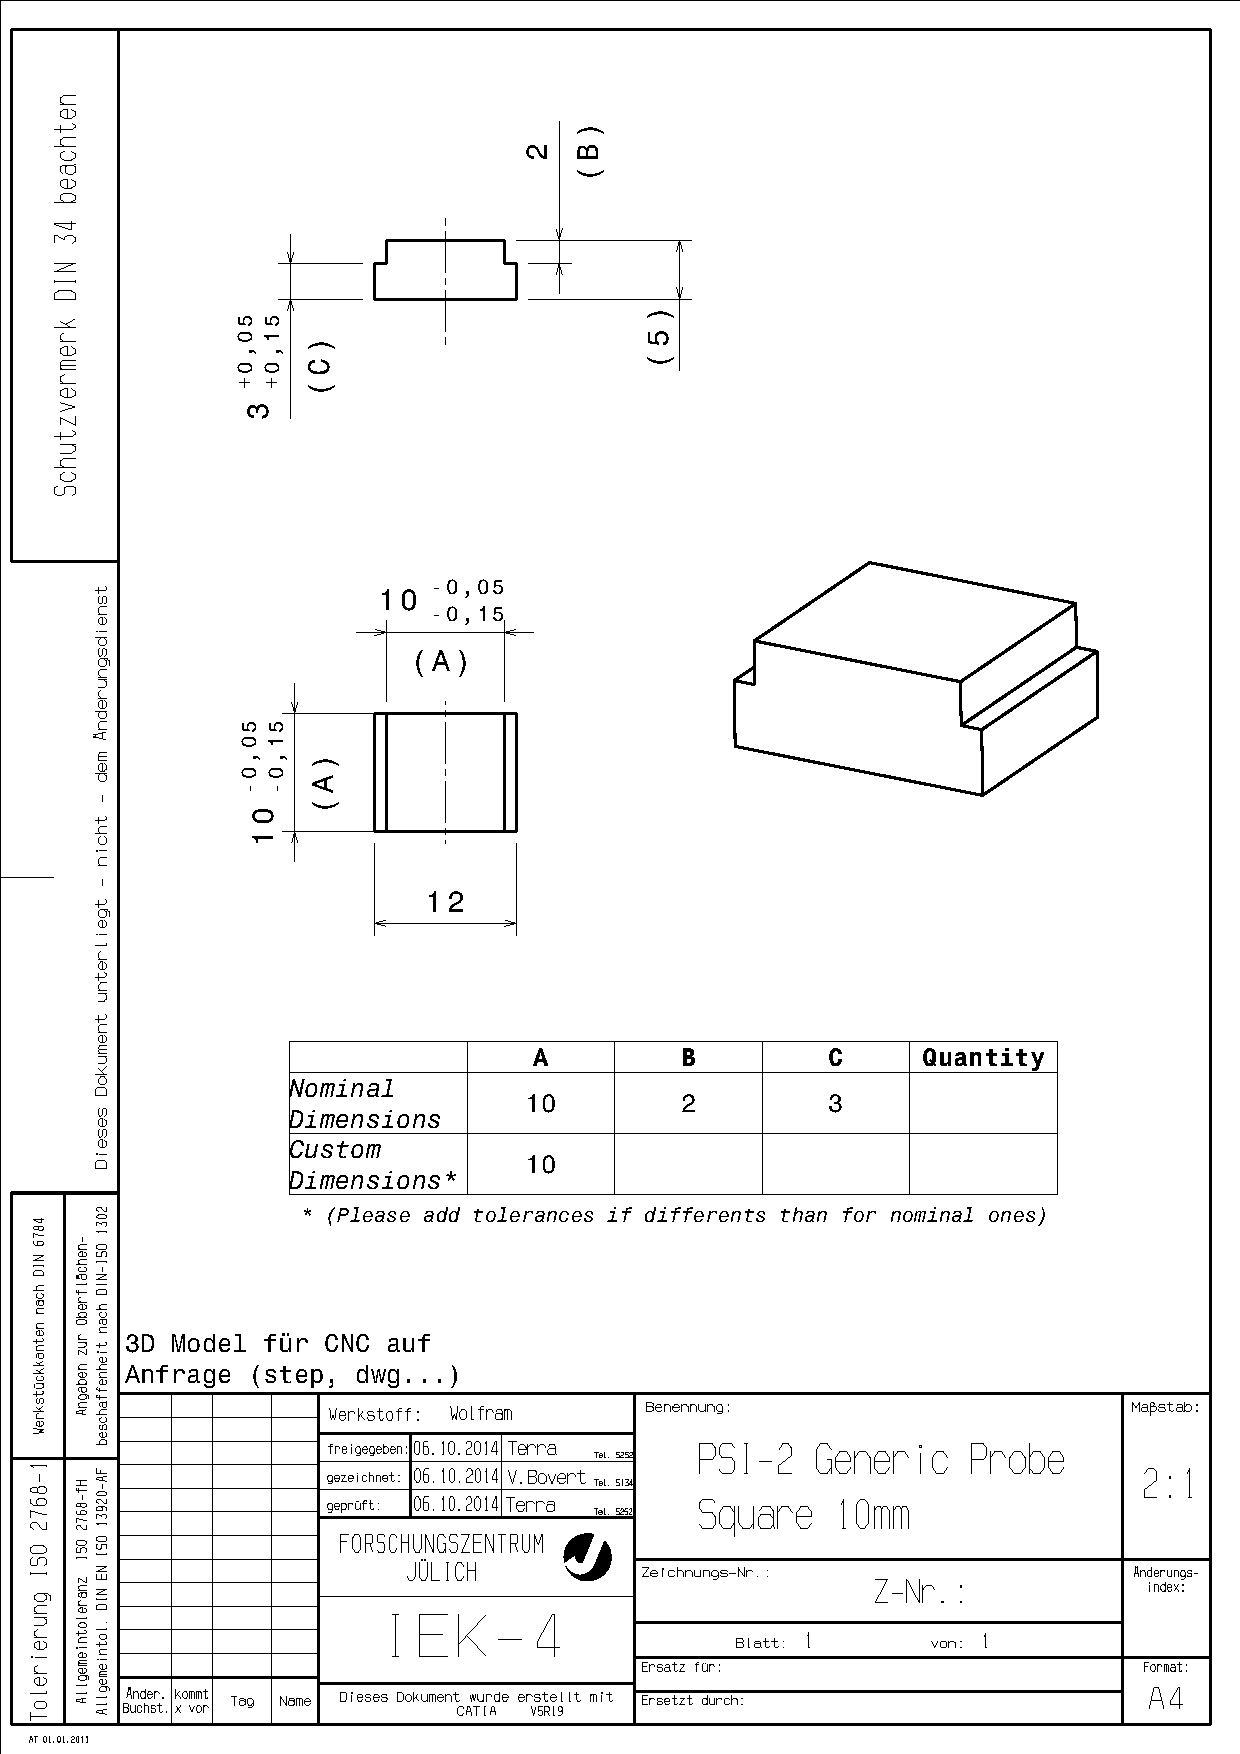
\includegraphics[height=0.33\textwidth]{figures/Sample.pdf}
    \includegraphics[height=0.33\textwidth]{figures/mask.pdf}
    \caption{The mask (right figure) is made out of tungsten and can contain 8 samples (left figure), 
    the 10x10mm top of the samples are coated with boron and attached in the mask such that it is facing towards    the plasma in the vessel}
    \label{fig:samples+mask}
\end{figure}
One may analyse boron-tungsten erosion by using neutral and ion beams,
mimicking actual IC,EC and IC+EC heated fusion devices, the obvious 
advantage being that the experiment is simpler with
easily chosen and controlled parameters.  But the disadvantage is that co-operative effects,
which may occur only when a plasma is present, will not be observed
\cite{McCRACKEN}. The TOMAS machine \cite{TOMAS} will be used as it is capable
of forming a toroidal plasma with pure ICRH discharge, thus introducing these
co-operative effects.  It is equiped with a monopole ICWC antenna which will be
set to operate at 50MHz, closely mimicking the 53MHz that will likely be used
at ITER.  The mask containing the samples (see figure \ref{fig:samples+mask})
is mounted on a movable arm which we'll position on top of the vessel.  
We'll modify the pressure in such a way that the
neutrals pressure (i.e the observed pressure during the discharge) is $10^{-5}$
mbar, closely mimicking what was the case in JET and will likely be the case in
ITER \cite{DOUAI}.
The exposures will be deuterium at different power levels (1.5kW, 3.5kW and
5.5kW), the thickness of the boron layer will be tracked by using ellipsometry
before and after on all samples and IBA+SEM (creating a hole using IBA and
scanning thickness using SEM) post mortem and on one control sample.
\section{Erosion estimation using neutrals}
\subsection{Explanation of the theory}
The erosion rates should be easy to measure, as such it should be short enough
to leave some boron intact but not too short as to have a statistically
significant reduction in thickness.  To this end an estimation of the
sputtering rate will be made prior to the discharge and the time under plasma
will be chosen accordingly. As the TOMAS machine's RFEA (Retarding Field Energy
Analyzer) is at the moment of writing unable to measure the ion distribution,
the only usable proxy to estimate the ideal time under load is the high
energy neutrals measured using the ToF-NPA (Time of Flight Neutral Particle
Analyzer) \cite{ToF-NPA} with some factor to account for the ions.
\noindent
\begin{figure}[ht]
    \centering
    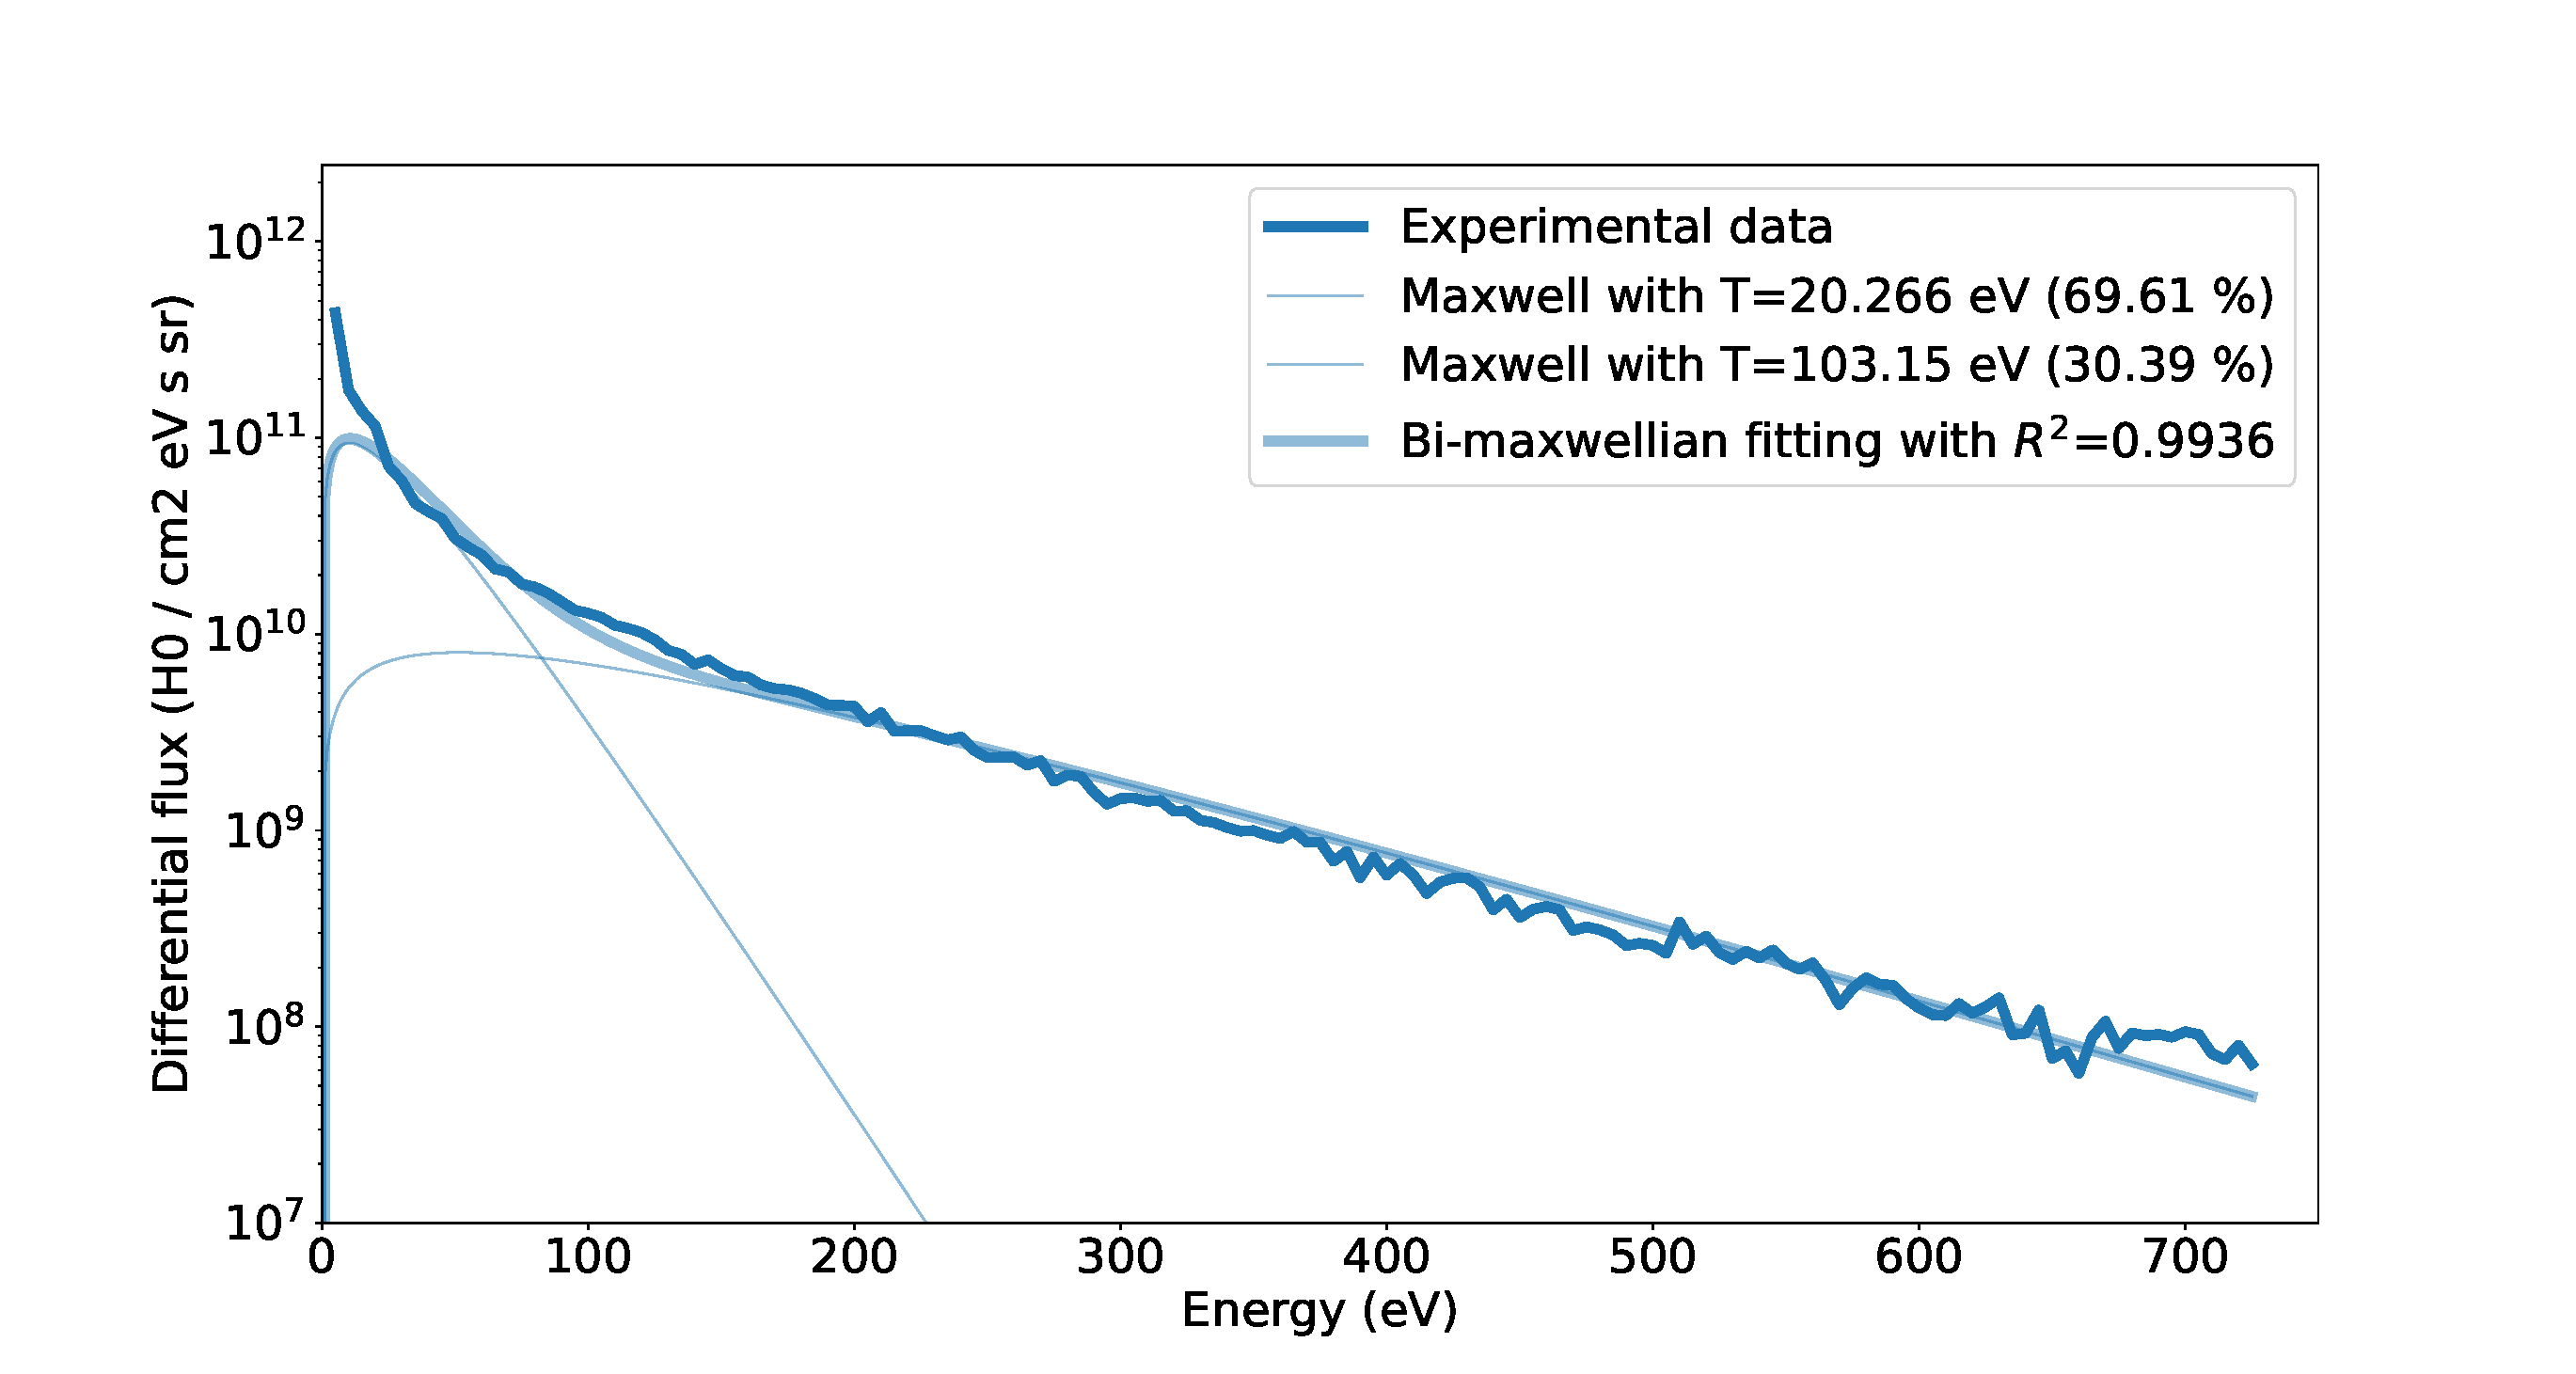
\includegraphics[width=0.7\textwidth]{figures/NPA_example.pdf}
    \caption{Our assumption behind the bi-maxwellian distribution is based on
        the characteristic that IC heating causes such a distribution in ions
        \cite{Bi-Maxwell} combined with the knowledge of rate coefficients for atomic charge
        exchange which is dominant at the observed kinetic energies \cite
        {McCRACKEN}, i.e the bi-maxwellian ions "transfer" their energies to the neutrals
        causing the same bi-maxwellian to be visible in the neutral energies.  
        Note that the $R^2$ parameter of the fitting on the graph
        is defined with the logarithmic difference to better emphesize the shape.}
    \label{fig:examplemeasurement}
\end{figure}\\
An example measurement made with the NPA is shown in figure
\ref{fig:examplemeasurement}. As the data is expressed as differential flux,
it lends itself to be easily manipulated into other quantities. One such manipulation
is using the following formula to transform it into an ersoion rate (m/s):
\begin{equation}
    S = \frac{2\pi}{N} \int_E Y(E)\partial\mathcal{F} (E) \text{dE}
    \label{eqn:ErosionRateFormal}
\end{equation}
With $Y(E)$ the yield of the neutrals on the material (i.e how many atoms of
the material get sputtered for every incoming neutral), $\partial\mathcal{F}(E)$ the
experimental differential flux as previously shown and N the number density.
The validity of this formula is quite straightforward to see as:
\begin{itemize}
    \item The NPA covers a certain solid angle, this has been accounted for as
        can be seen in the unit of the example experiment (/sr meaning per
        steradian), we can get an approximation for the average
        flux in the vessel by assuming homogeneity and thus multiplying this
data by $2\pi$ steradians. 
    \item The differential flux of particles in an energy bin surrounding $E$ causes sputtering, to get this
        sputtering rate we multiply by the yield $Y$ at that energy as it's defined to be the
        outgoing atoms per incoming, we integrate over all energies to get the
        full contribution. 
    \item The number density of the target $N$ dictates how the amount of
        outgoing atoms relates to the decrease in thickness, this can be seen from the units.
\end{itemize}
In the analysis software equation \ref{eqn:ErosionRateFormal} is used in the discrete form,
summing over the energy bins:
\begin{equation}
S = \frac{2\pi}{N}\sum_{E_0}^{E_{\text{max}}} Y(E)\partial\mathcal{F}(E)\Delta\text{E}
    \label{eqn:ErosionRateFinite}
\end{equation}
Where we may get the yield $Y(E)$ using the software RustBCA\cite{RustBCA},
assuming ions to behave the same as neutrals (as the samples aren't charged,
this should give a negligable discrepancy) with parameters from Wolfgang Eckstein's
book \cite{eckstein2013computer}, assuming perpendicular impingement\footnote{note that
assuming a distribution such as $\cos(\theta)^2$ doesn't change the result by more than $10\%$}.
\subsection{Calculated estimates}
\section{Experimental Results}
\section{Calculation of PFM Normit relations}

%----------------------------------------------------------------------------------------
%	REFERENCE LIST
%----------------------------------------------------------------------------------------
\bibliographystyle{iopart-num}
\bibliography{Bibliography/sources}
%----------------------------------------------------------------------------------------

\end{document}
